\documentclass[12pt]{article}
\usepackage{graphicx}
\usepackage{amsmath}
\usepackage{mathtools}
\usepackage{gensymb}

\newcommand{\mydet}[1]{\ensuremath{\begin{vmatrix}#1\end{vmatrix}}}
\providecommand{\brak}[1]{\ensuremath{\left(#1\right)}}
\providecommand{\norm}[1]{\left\lVert#1\right\rVert}
\newcommand{\solution}{\noindent \textbf{Solution: }}
\newcommand{\myvec}[1]{\ensuremath{\begin{pmatrix}#1\end{pmatrix}}}
\let\vec\mathbf

\begin{document}
\begin{center}
\section*{CHAPTER 7 - COORDINATE GEOMETRY}

\end{center}
\section*{Excercise 7.2}

Q7.Find the coordinates of point A, where AB is the diameter of a circle where the center is (2,-3) and B is the point (1,4):

\solution
\begin{enumerate}
\item The coordinates B and center C are given, where:
	\begin{align}
	\vec{B} = \myvec{
		1\\
	    4\\
		},
	\vec{C} = \myvec{
	    2\\
	   -3\\
		},
	\end{align}
Let us assume the coordinates of A. Now, C is the center which is midpoint of line AB and B is one of the coordinate of diameter AB of a circle.
		
Hence,	
	\begin{align}
	\vec{C} = \frac{\vec{A+B}}{2} \\
	2\vec{C} &= \vec{A}+\vec{B} \\
	\vec{A} &= 2\vec{C}-\vec{B} \\
	\vec{A} &= 2\myvec{2\\-3\\}-\myvec{1\\4\\} \\
	\vec{A} &= \myvec{4\\-6\\}-\myvec{1\\4\\} \\
	\vec{A} &= \myvec{4-1\\-6-4\\} \\	
	\vec{A} &= \myvec{3\\-10\\}	
	\end{align}       
    Therefore,the coordinates of A for value for given point $\vec{B(1,4)}$ and center $\vec{C(2,-3)}$ given by $\vec{A(3,-10)}$.	
\hspace{5mm}
\begin{figure}[!h]
\begin{center}	
	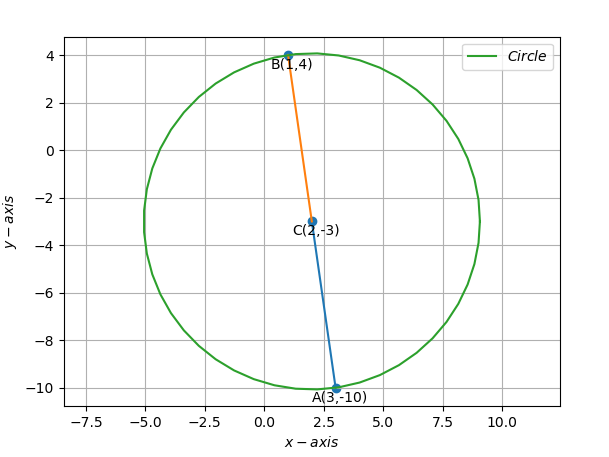
\includegraphics[width=\columnwidth]{./figs/Vector1.png}
\end{center}
\caption{Circle for the given coordinates}
\label{fig:Fig}
\end{figure}
\end{enumerate}
\end{document}
	
